\documentclass[a4paper,12pt]{article}

\usepackage[T2A]{fontenc}
\usepackage[utf8]{inputenc}
\usepackage[english,russian]{babel}

\usepackage{amsmath, amssymb} 
\usepackage{geometry} 
\geometry{top=2cm, bottom=2cm, left=2cm, right=2cm}
\usepackage{graphicx} 
\usepackage{float} 
\usepackage{blkarray} 
\usepackage{booktabs}
\usepackage{caption}
\usepackage{subcaption}

\begin{document}

\section{Минимальный ДКА}

Таблица классов эквивалентности для обоснования минимальности.

\begin{table}[h!]
\centering
\small
\begin{blockarray}{lcccccccccccccc}
 & c & bab & ab & bba & a & \varepsilon & cac & ac & cb & ccbb & cbb & bb & b & ba \\
\begin{block}{l[cccccccccccccc]}
1  & 1 & 1 & 0 & 0 & 0 & 1 & 0 & 0 & 0 & 0 & 0 & 0 & 0 & 1 \\
2  & 0 & 1 & 0 & 0 & 0 & 0 & 0 & 0 & 0 & 0 & 0 & 0 & 0 & 0 \\
3  & 0 & 1 & 1 & 0 & 0 & 0 & 0 & 0 & 0 & 0 & 0 & 0 & 0 & 0 \\
4  & 0 & 0 & 0 & 1 & 0 & 0 & 0 & 0 & 0 & 0 & 0 & 0 & 1 & 0 \\
5  & 0 & 0 & 1 & 0 & 1 & 0 & 0 & 0 & 0 & 0 & 0 & 0 & 0 & 0 \\
6  & 0 & 1 & 0 & 1 & 0 & 1 & 1 & 0 & 0 & 1 & 0 & 1 & 1 & 1 \\
7  & 0 & 0 & 0 & 0 & 0 & 0 & 1 & 0 & 0 & 0 & 0 & 0 & 0 & 0 \\
8  & 0 & 0 & 0 & 0 & 0 & 0 & 0 & 1 & 0 & 0 & 0 & 0 & 0 & 0 \\
9  & 1 & 0 & 0 & 0 & 0 & 0 & 0 & 0 & 1 & 0 & 1 & 0 & 0 & 0 \\
10 & 0 & 1 & 1 & 1 & 1 & 1 & 1 & 0 & 0 & 1 & 0 & 1 & 1 & 1 \\
11 & 0 & 0 & 0 & 0 & 0 & 0 & 0 & 1 & 0 & 0 & 1 & 0 & 0 & 0 \\
12 & 0 & 0 & 0 & 0 & 0 & 0 & 0 & 0 & 0 & 0 & 0 & 1 & 0 & 0 \\
13 & 0 & 0 & 0 & 1 & 0 & 0 & 0 & 0 & 0 & 0 & 0 & 1 & 1 & 0 \\
14 & 0 & 1 & 0 & 0 & 0 & 0 & 0 & 0 & 0 & 0 & 0 & 0 & 0 & 1 \\
\end{block}
\end{blockarray}
\end{table}

\begin{figure}[H]
    \centering
    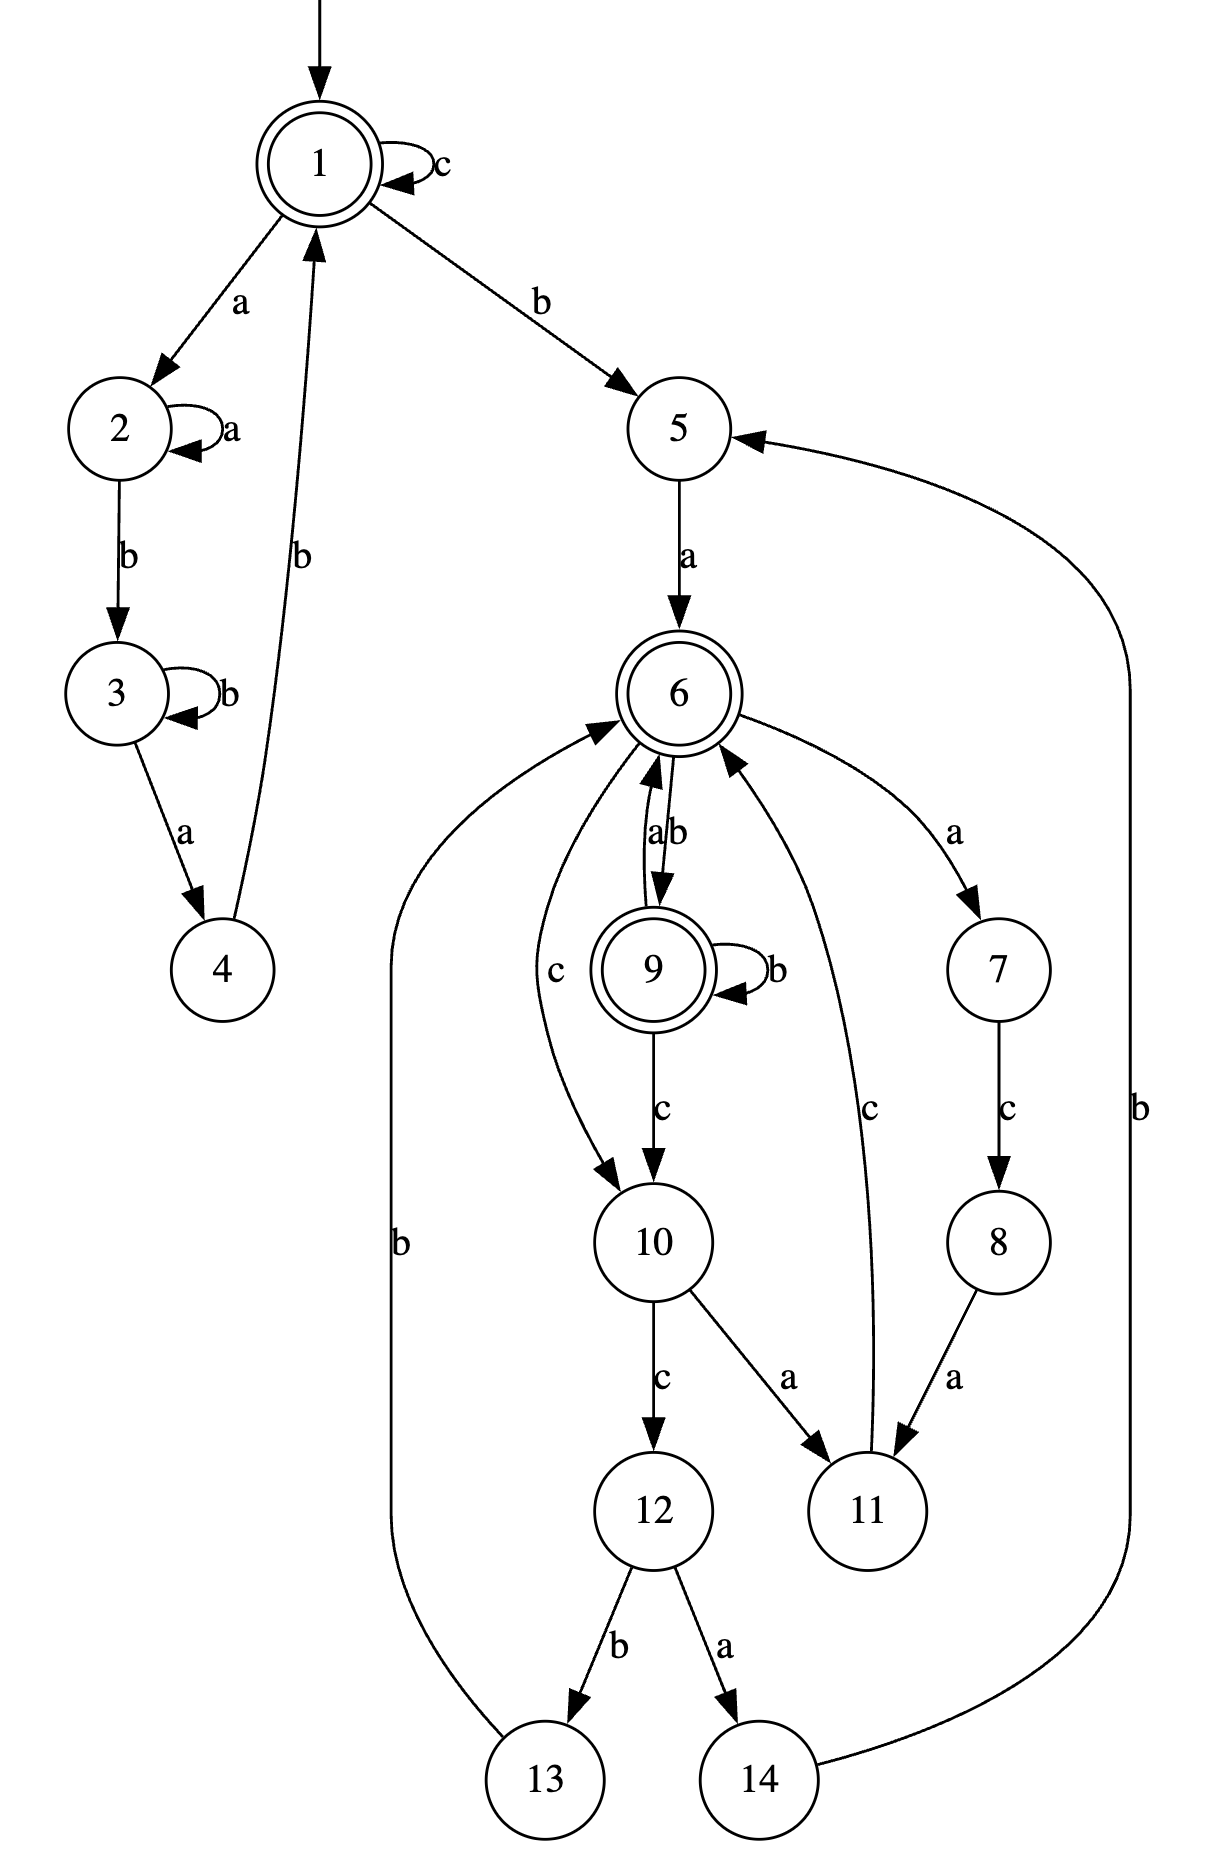
\includegraphics[width=0.8\linewidth]{mindfa.png}
    \caption{Граф минимального ДКА}
    \label{fig:mindfa}
\end{figure}

\newpage

\section{Возможно малый НКА и ПКА}

\subsection{Матрица для НКА}
\begin{table}[h!]
\centering
\renewcommand{\arraystretch}{1.3}
\begin{tabular}{|l|c|c|c|c|c|c|c|c|c|}
\hline
 & caba & c & b & a & cac & $\varepsilon$ & bb & ba & ac \\ \hline
bac & 1 & 0 & 0 & 0 & 0 & 0 & 0 & 0 & 1 \\ \hline
baca  & 0 & 1 & 0 & 0 & 0 & 0 & 0 & 0 & 0 \\ \hline
ba    & 0 & 0 & 1 & 0 & 1 & 1 & 1 & 1 & 0 \\ \hline
b     & 0 & 0 & 0 & 1 & 0 & 0 & 0 & 0 & 0 \\ \hline
baa   & 0 & 0 & 0 & 0 & 1 & 0 & 0 & 0 & 0 \\ \hline
$\varepsilon$ & 0 & 0 & 0 & 0 & 0 & 1 & 0 & 1 & 0 \\ \hline
bacc  & 0 & 0 & 0 & 0 & 0 & 0 & 1 & 0 & 0 \\ \hline
bacca & 0 & 0 & 0 & 0 & 0 & 0 & 0 & 1 & 0 \\ \hline
baac  & 0 & 0 & 0 & 0 & 0 & 0 & 0 & 0 & 1 \\ \hline
\end{tabular}
\caption{Верхняя часть автомата}
\end{table}

\begin{table}[h!]
\centering
\renewcommand{\arraystretch}{1.3}
\begin{tabular}{|l|c|c|c|c|}
\hline
 & $\varepsilon$ & b & ab & bab \\ \hline
$\varepsilon$ & 1 & 0 & 0 & 0 \\ \hline
aba           & 0 & 1 & 0 & 0 \\ \hline
ab            & 0 & 0 & 1 & 0 \\ \hline
a             & 0 & 0 & 0 & 1 \\ \hline
\end{tabular}
\caption{Нижняя часть автомата}
\end{table}


\begin{figure}[H]
    \centering
    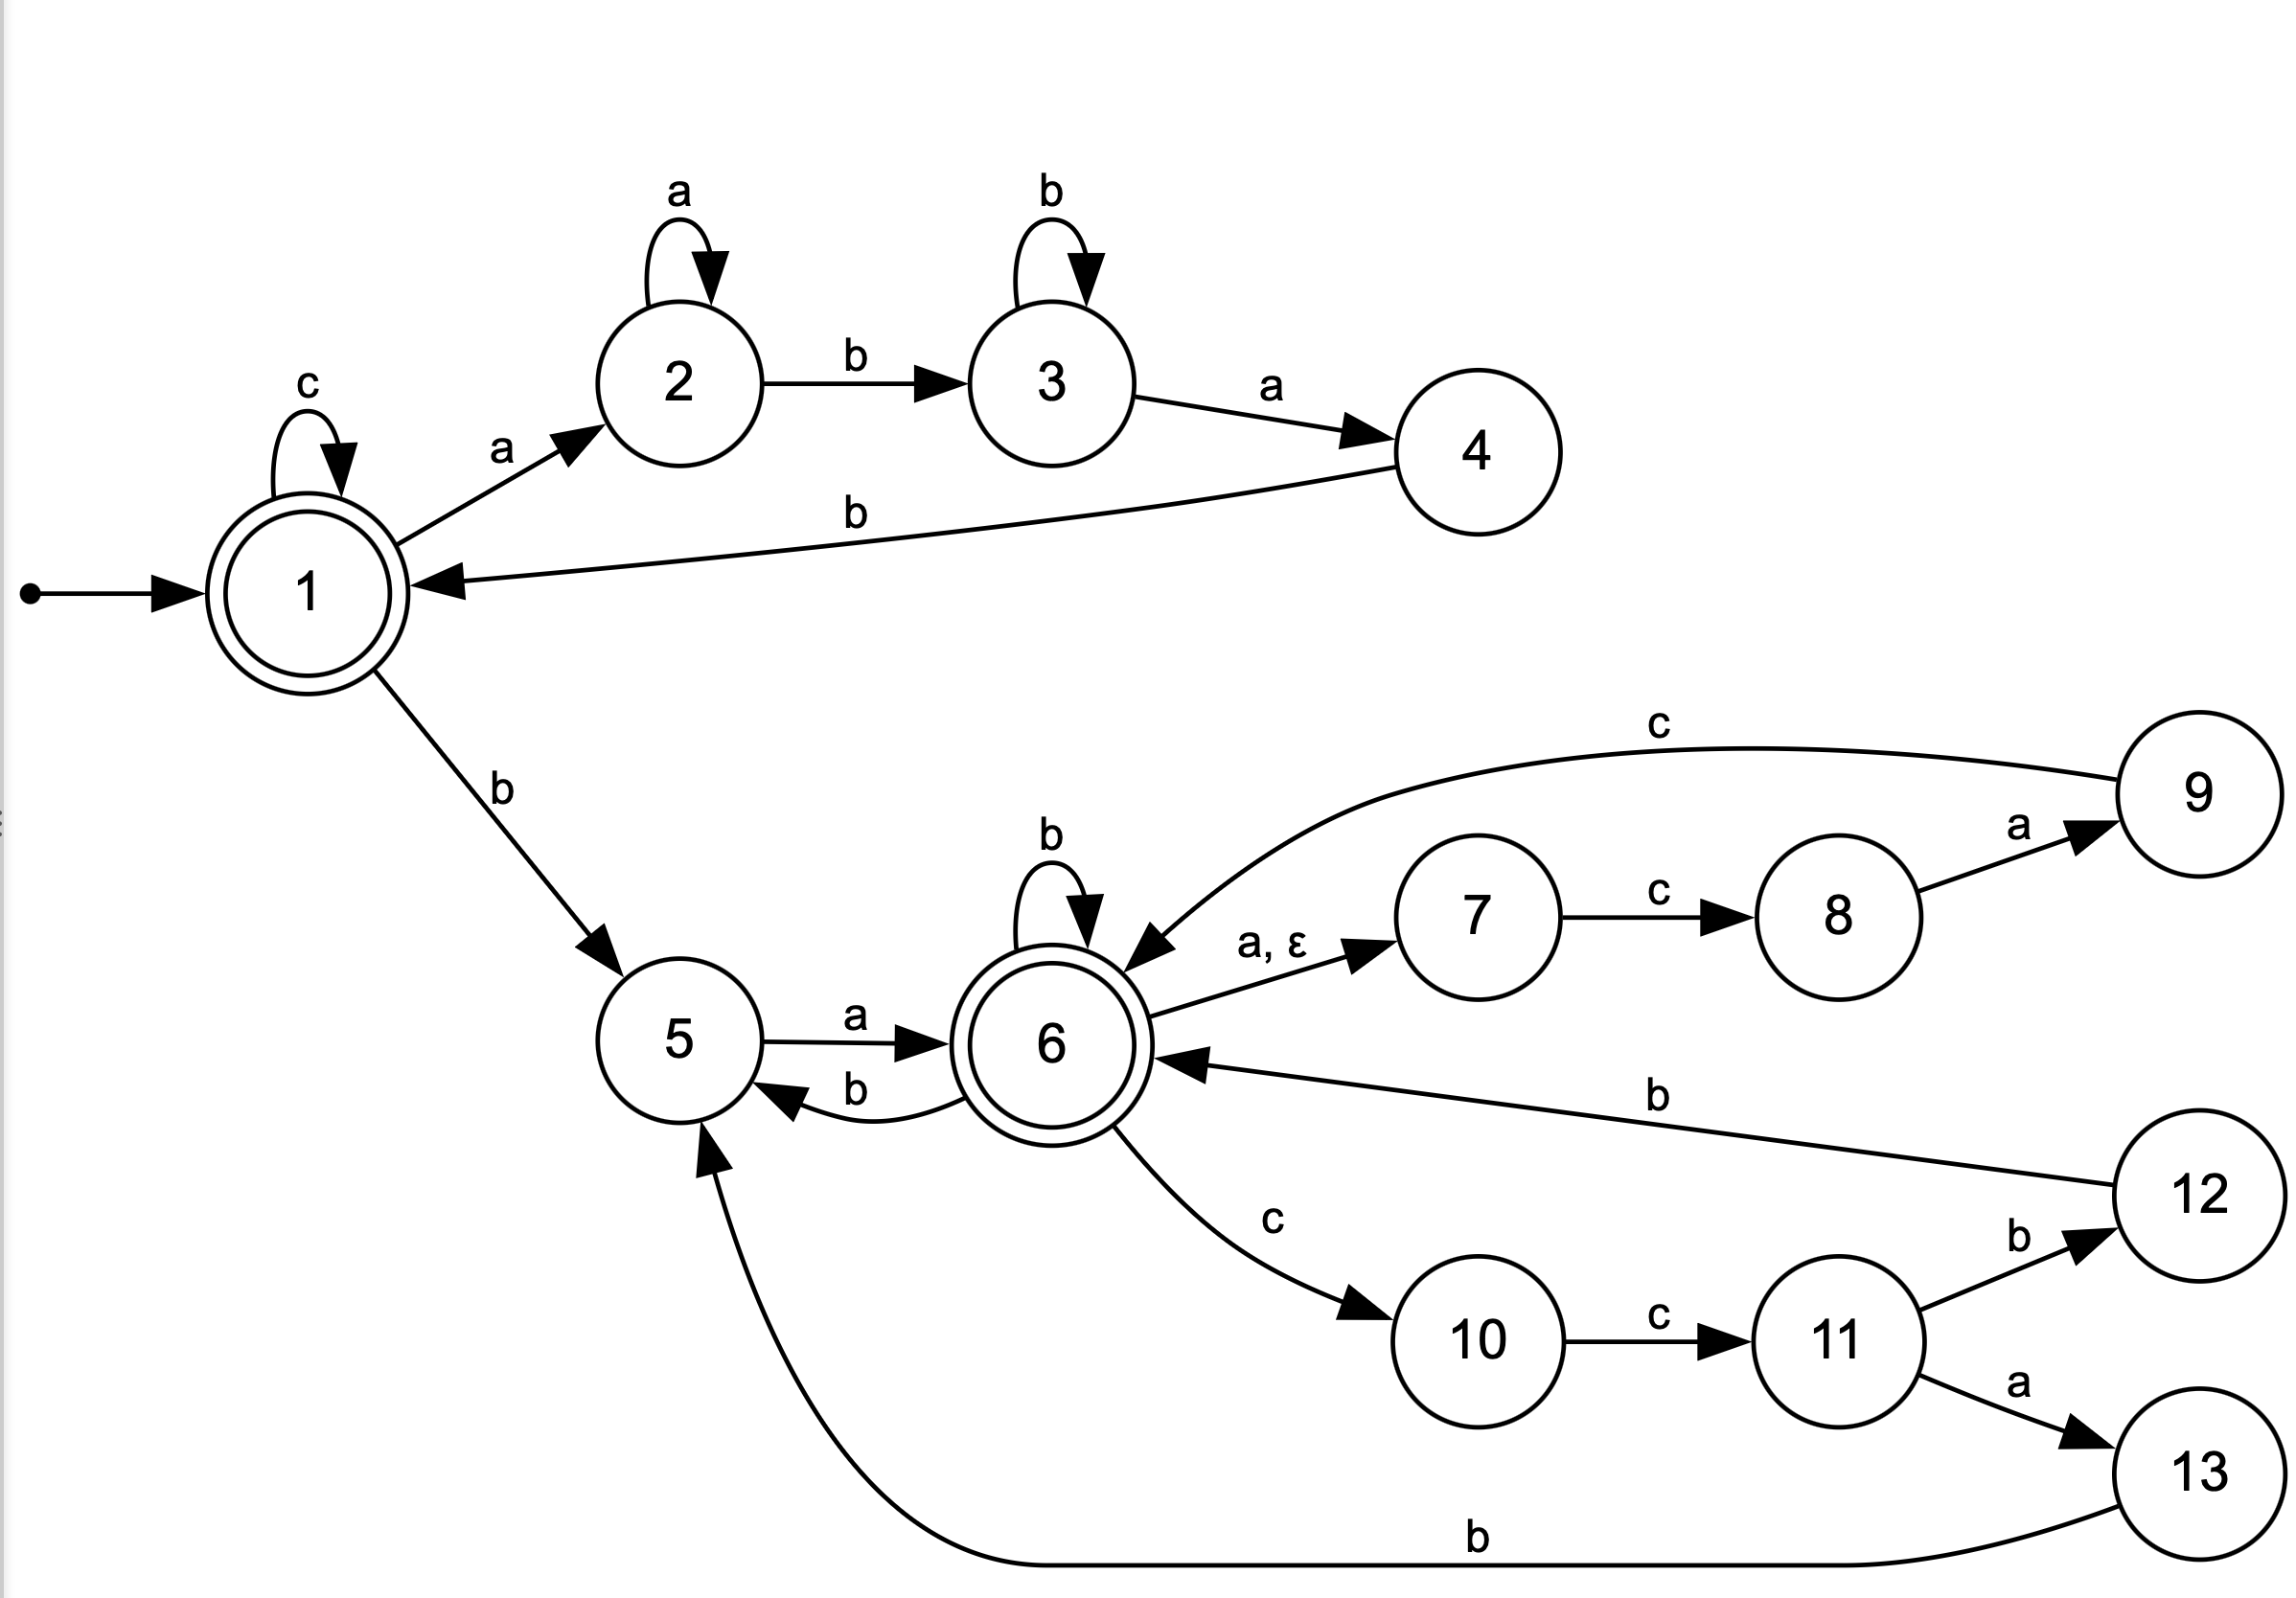
\includegraphics[width=0.8\linewidth]{nfa.png}
    \caption{Граф НКА}
    \label{fig:nfa}
\end{figure}

\subsection{Матрица для ПКА}
\begin{table}[h!]
\centering
\renewcommand{\arraystretch}{1.5} % Добавляет немного пространства между строками для читаемости
\begin{tabular}{|l|c|c|c|c|c|c|}
\hline
 & c & a & b & $\varepsilon$ & ba & bab \\ \hline
bab   & 0 & 1 & 1 & 1 & 1 & 1 \\ \hline
ba    & 0 & 0 & 1 & 1 & 1 & 1 \\ \hline
$\varepsilon$ & 1 & 0 & 0 & 1 & 1 & 1 \\ \hline
bacca & 0 & 0 & 0 & 0 & 1 & 1 \\ \hline
a     & 0 & 0 & 0 & 0 & 0 & 1 \\ \hline
aba   & 0 & 0 & 1 & 0 & 0 & 0 \\ \hline
\end{tabular}
\end{table}

\begin{figure}[H]
    \centering
    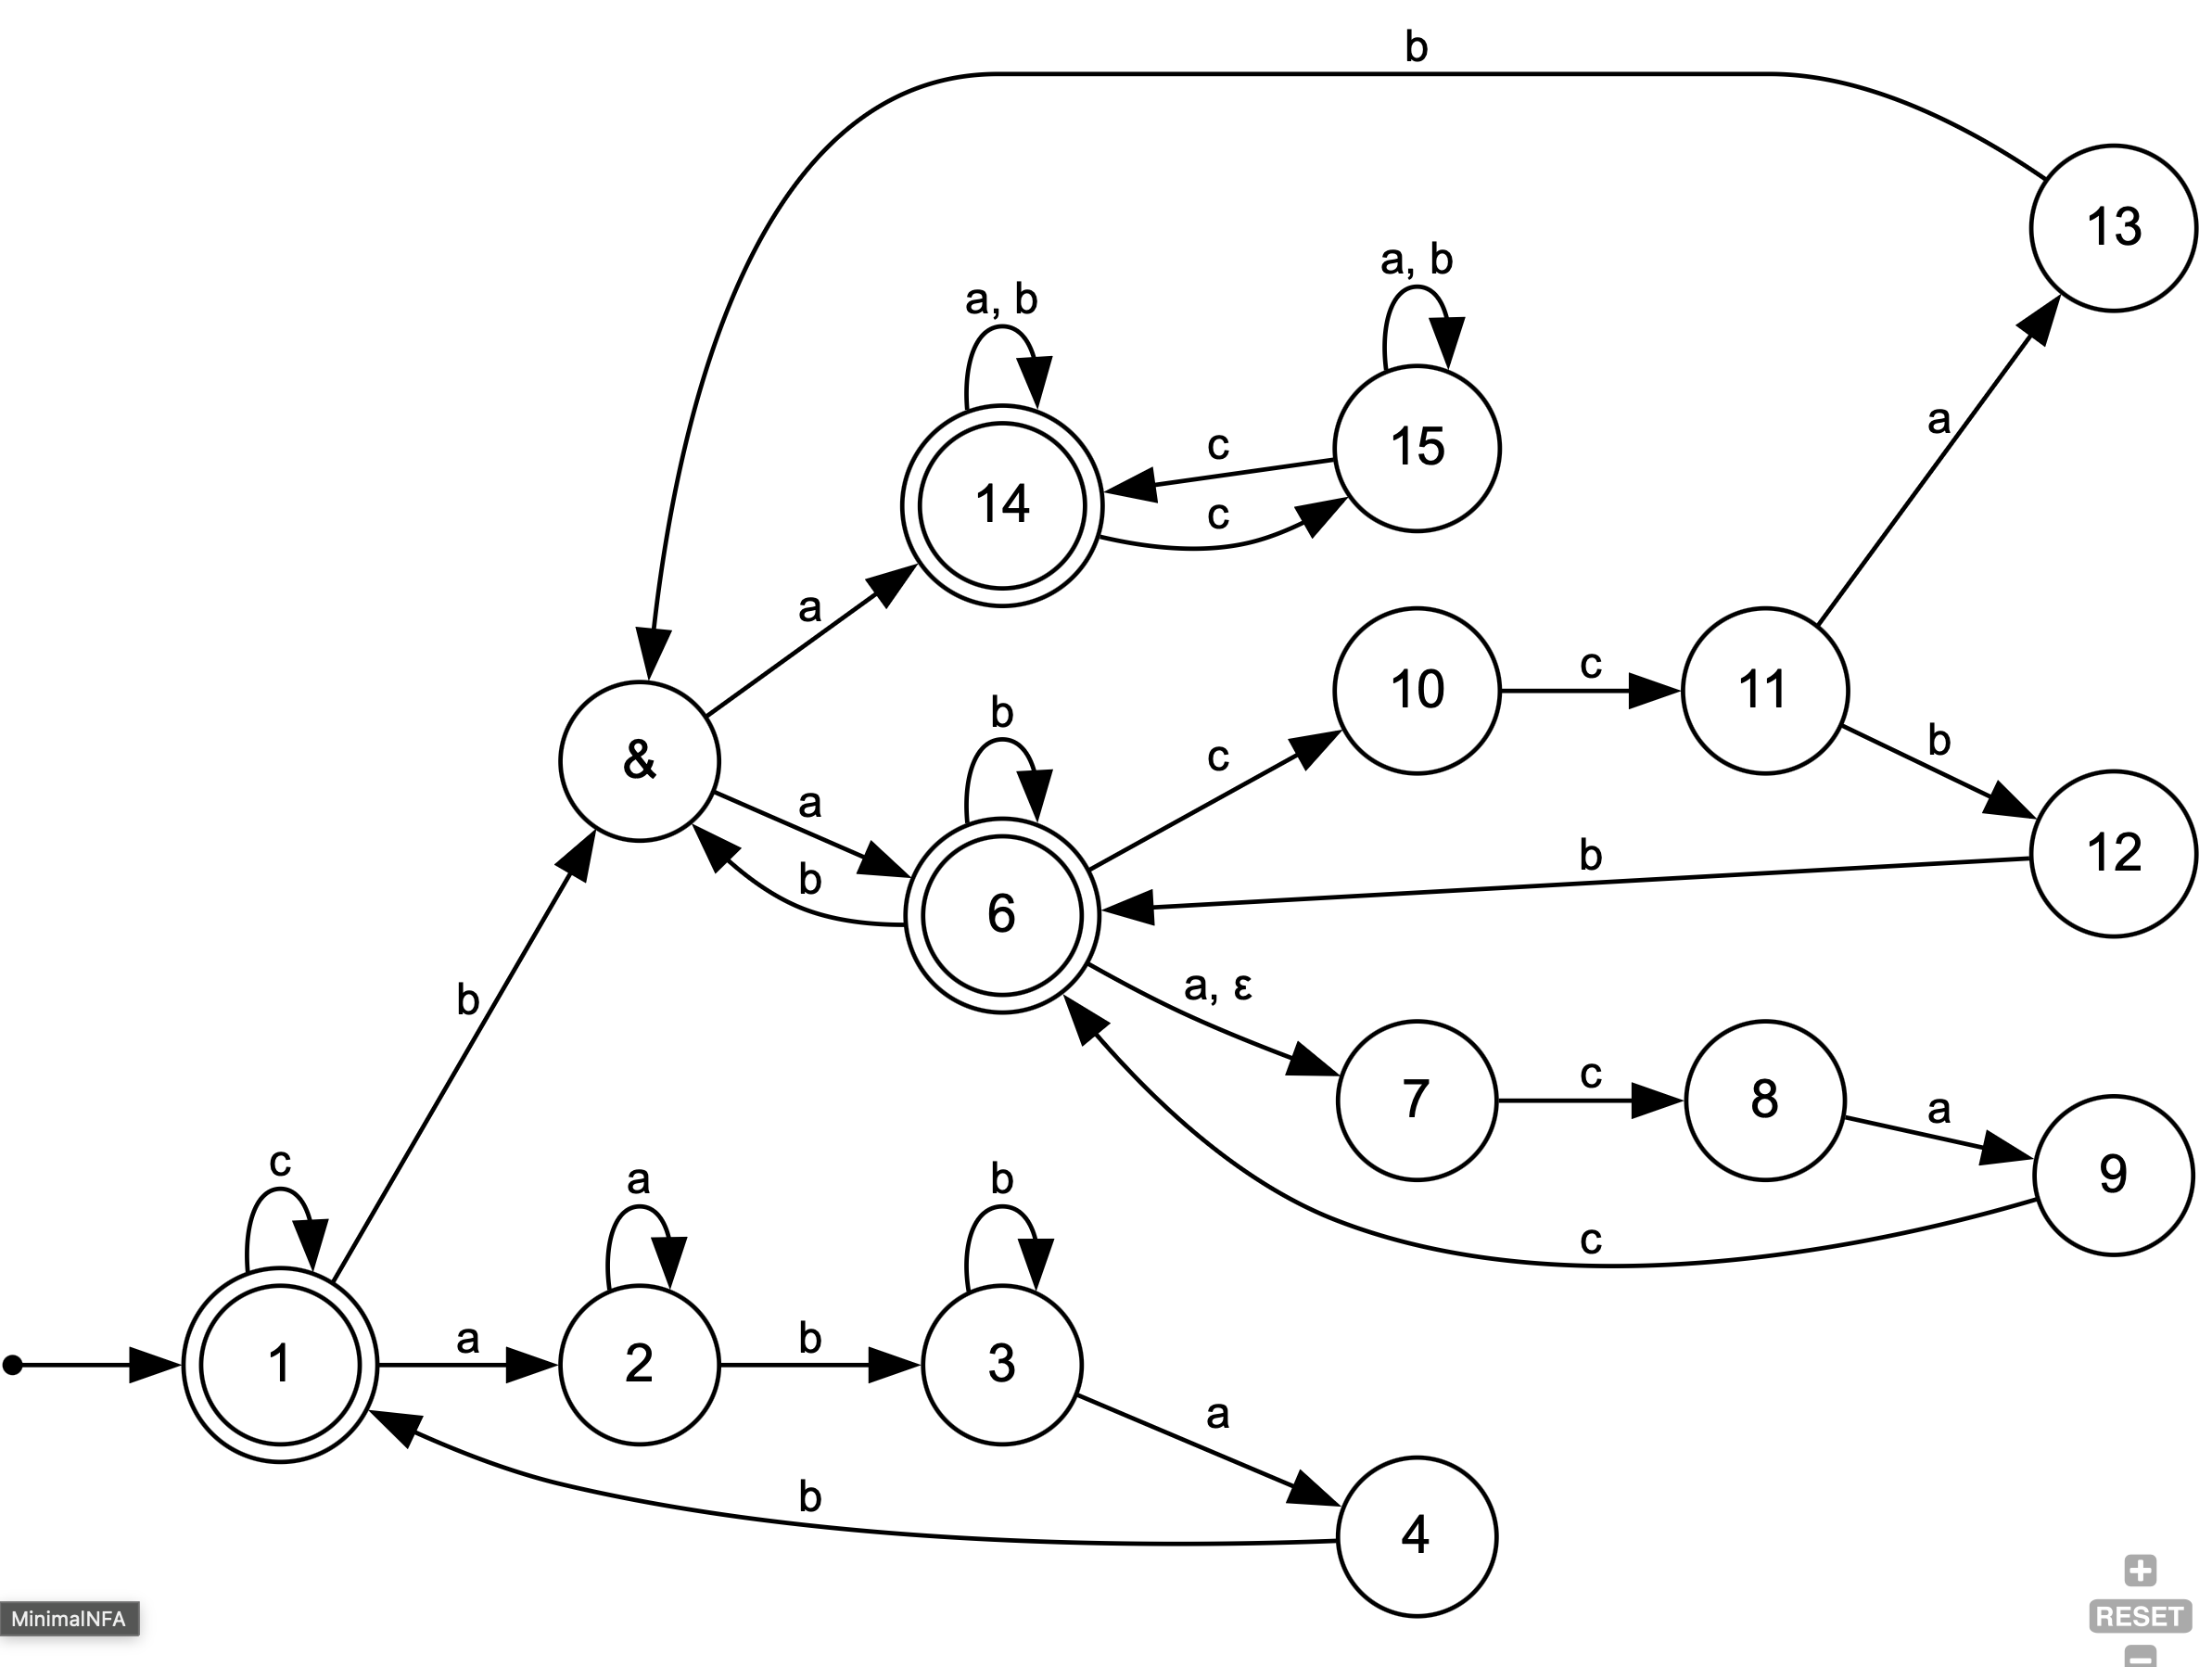
\includegraphics[width=0.8\linewidth]{pka.png}
    \caption{Граф ПКА}
    \label{fig:pka}
\end{figure}

\section{Расширенное регулярное выражение}

Расширенное регулярное выражение, распознающее тот же язык:

\begin{equation*}
    \wedge \left( a^+ b^+ ab \mid c \right)^* \left( ba \left( a?cac \mid ba? \mid cc(bb|aba) \right)^* \right)? \$
\end{equation*}

\end{document}
